\chapter{Web Services}
\setcounter{page}{1}
	\section{Support for the requirements}
		\vspace{5mm}
	    \begin{multicols}{2}
		\paragraph{}
			
		Service-oriented applications (SOA) that communicate across the web	is a mechanism for supporting distributed computing 
		with the intent of exposing services that typically cannot be exposed by conventional web implementations.
		\newline  
		\newline 
		A conventional web implementation using the Hyper Text Transfer Protocol (http) is a mechanism to provide web content to web browsers.
		In the event of a developer wanting to communicate with a service using conventional 'application' means, such as method invocation, routines
		etc, an application server must be used.  This application server handles the transfer of invocations and therein serialized information to the 
		service or process which the application server exposes.  This allows for almost transparent access to services resources by letting the application
		server do all the heavy lifting.  Unlike in a typical situation of opening a socket and sender raw information down the socket. 
		\newline

		For the assignment of a service computational calculator exposes an interface via a service definition contract or interface; defined in the 
		Web Service Description Language (WSDL).  This contract which clients subscribe provide the client with the means to interface and communicate 
		correctly with the service.  
	
		\end{multicols}
		
		\begin{figure}[h!]
			\centering
			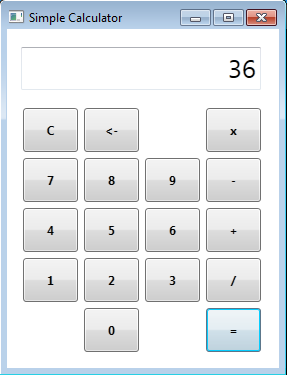
\includegraphics[scale=0.5]{figures/calc.png}
			\caption{Calculator}
		\end{figure}

		\vspace{5mm}
	    \begin{multicols}{2}
		\paragraph{}
		
		As the service implemented as web service, other clients can utilize the service as long as to conform to the specification of the contract.
		Orchestration can be catered for by design as the application and can be utilized as part of the web work flow.
		 
		
		\end{multicols}